\documentclass[letterpaper,11pt]{article}
\usepackage{xeCJK}
\usepackage{bm}
\usepackage{geometry}
\usepackage{amssymb}
\usepackage{amsmath}
\usepackage[cal=boondoxo, scr=dutchcal]{mathalfa}
\usepackage{multirow}
\usepackage[unicode, CJKbookmarks=true]{hyperref}

\numberwithin{equation}{section}

\geometry{a4paper,left=2cm,right=2cm,top=2cm,bottom=2cm}

\usepackage{setspace}
\setstretch{1.1}
\setlength{\parskip}{0.1\baselineskip}

\usepackage{graphicx}
\usepackage{caption}
\renewcommand{\figurename}{图}
\renewcommand{\tablename}{表}

\usepackage[backend=biber, style=ieee]{biblatex}
\addbibresource{ref.bib}

\begin{document}

\title{AI分享}
\author{张驰}
\maketitle

\begin{figure}[htbp]
    \centering
    
\includegraphics[width=1\textwidth]{../../assets/imgs/ai_share/bg.jpg}
    \caption*{黑客帝国动画版(2003)海报}
\end{figure}

\section{引子}

近年,AI对不少行业都形成了一定的影响,大家对AI的热情也愈发高涨。
希望通过这篇文章以简单直观的方式介绍大模型领域的常见概念、各种时髦的名词及新兴技术(像是AI Agent、Function Call、MCP等),帮助大家了解当前的热点技术与工具,当工作中涉及AI时,可以有一定的判断。
这篇文章主要讲解大模型相关技术与工具的背景、功能与使用场景,对于这些背后的原理只做简单阐述,如有兴趣可以进一步阅读参考文献。

\section{大模型的工作原理}

在阐述大模型相关的技术与工具前,需要大家首先对大模型的工作原理有一定了解。
对于大模型的详细工作原理可参阅文献\cite{alammar2018transformer}。
其实大模型的工作原理很简单,就是四个字“文字接龙”,大模型根据输入的Prompt计算出下一个可能的字或词,再用此Prompt附加上新产生的字或词作为大模型新的输入,重复此过程直至得到完整的结果,大模型的简易工作原理如图\ref{fig:llm-workflow}所示:

\begin{figure}[!htbp]
    \centering
    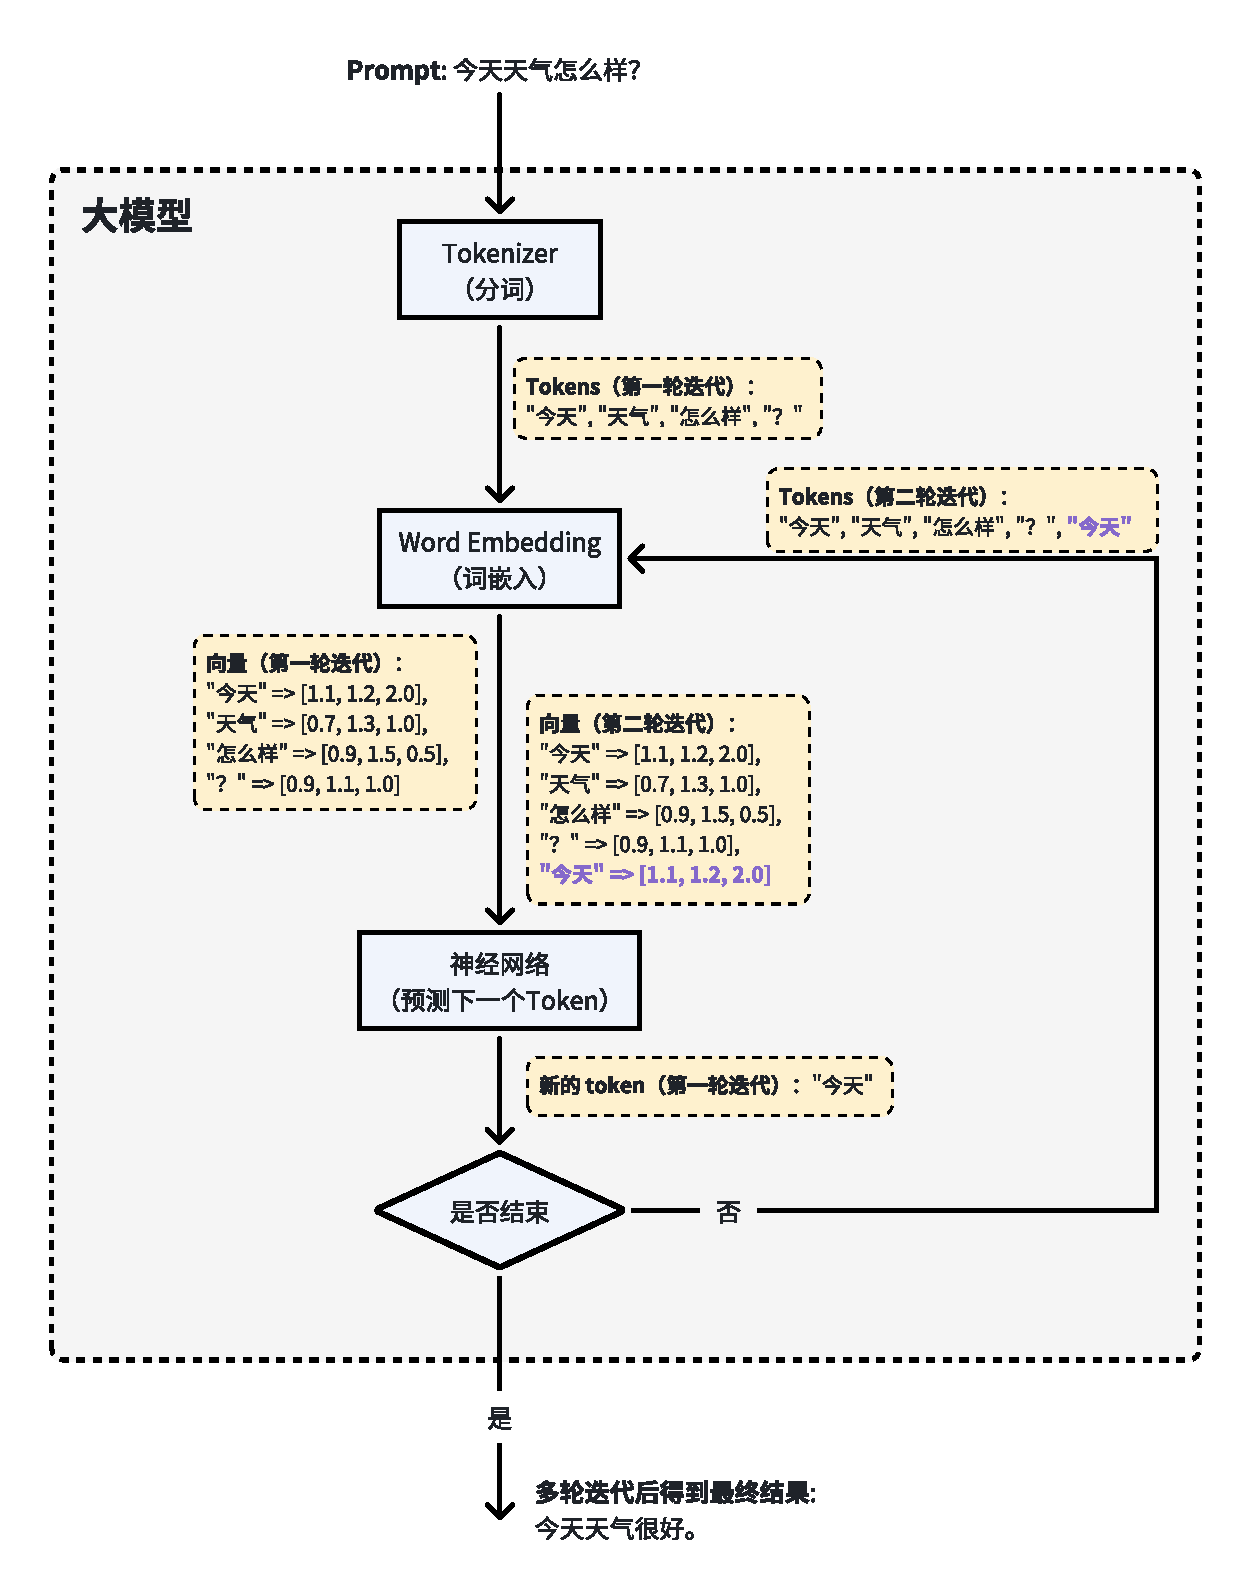
\includegraphics[width=0.6\textwidth, height=12cm, keepaspectratio]{../../assets/imgs/ai_share/llm_workflow.pdf}
    \caption{大模型的工作流程}
    \label{fig:llm-workflow}
\end{figure}

举个例子,如果向大模型输入Prompt“今天天气怎么样?”,大模型大概会按以下流程进行工作并输出结果:
\begin{enumerate}
    \item 分词\footnote{分词是自然语言处理中非常重要的一步,目的是将连续的文本按语义或语法规则切分成独立的词语单元,最近大名鼎鼎的DeepSeek V3模型采用的是Byte-level BPE分词算法。另外,在进行分词前,通常需先对文本进行归一化(Normalize)处理,目的是将不同形式、书写习惯或字符表示的文本统一为一致的格式,以避免因表面形式的差异导致分词错误。对于分词的详细可参阅文献\cite{glan2023tokenizer},另外Hugging Face也提供了一个Tokenizer的Rust实现\cite{huggingface_tokenizers}。},大模型首先对Prompt进行分词处理,将其分解为token序列“今天”、“天气”、“怎么样”与“?”;
    \item 词嵌入\footnote{这里大家可能会有疑问,这个功能是将token转化为向量,那为什么不叫作“向量化”,而是叫作“词嵌入”呢?“词嵌入”这个词最早出现于Google AI在2013年提出的Word2vec模型\cite{mikolov2013efficientestimationwordrepresentations},词嵌入旨在将每个词赋予唯一的量化值,并且语义较近的词的量化值间的距离应当近,语义较远的词的量化值间的距离应当远,另外每个词在不同的上下文中可能会有不同的语义,为了承载语义的复杂性,量化值通常是多维向量,这里推荐阅读文献\cite{constantine2023wordembedding}。},大模型随后对token进行词嵌入处理,将每个token转化为一个向量,比如“今天”被转化为向量$[1.1, 1.2, 2.0]$;
    \item 预测,大模型再将向量输入至神经网络进行计算得到一个新的token,如“今天”;
    \item 附加,大模型再将新的token附加至之前的token序列,得到新的token序列“今天”、“天气”、“怎么样”、“?”与“今天”;
    \item 重复步骤2-4直至得到最终结果。
\end{enumerate}

\printbibliography[title={引用}]

\end{document}